\documentclass[tikz,border=6pt]{standalone}
\usepackage{amsmath,amssymb,mathtools,physics,bm,nicefrac,wasysym}
\usepackage{xcolor}

\definecolor{colone}{RGB}{180,60,60}
\definecolor{coltwo}{RGB}{60,110,180}
\definecolor{colthree}{RGB}{60,140,80}

\definecolor{accent}{HTML}{A13D2C}
\definecolor{accent2}{HTML}{2B5F6B}
\definecolor{muted}{HTML}{5A564F}
\definecolor{panel}{HTML}{F8F6F0}
\definecolor{linecol}{HTML}{D8D2C4}
\definecolor{ink}{HTML}{1E1C1A}
\definecolor{astroblue}{HTML}{1B4F72}
\definecolor{astrodark}{HTML}{17202A}
\definecolor{sunyellow}{HTML}{E8A33D}

\usetikzlibrary{calc,arrows.meta,positioning,decorations.pathreplacing,decorations.markings,angles,quotes,shapes.geometric}
\usepackage{tikz-3dplot}

\newcommand{\vecr}{\vec r}
\newcommand{\vecL}{\vec L}
\newcommand{\vecA}{\vec A}
\newcommand{\vecf}{\vec f}
\newcommand{\vecF}{\vec F}
\newcommand{\vecp}{\vec p}
\newcommand{\avg}[1]{\left\langle #1\right\rangle}
\newcommand{\vecx}{\vec x}
\newcommand{\hatn}{\hat n}
\newcommand{\rhat}{\hat r}
\newcommand{\phihat}{\hat\phi}
\newcommand{\thetahat}{\hat\theta}
\newcommand{\note}[1]{\textcolor{blue!60!black}{\textit{[#1]}}}

\newcommand{\LST}{\mathrm{LST}}
\newcommand{\GST}{\mathrm{GST}}
\newcommand{\GMST}{\mathrm{GMST}}
\newcommand{\GAST}{\mathrm{GAST}}
\newcommand{\LMST}{\mathrm{LMST}}
\newcommand{\LAST}{\mathrm{LAST}}
\newcommand{\UT}{\mathrm{UT}}
\newcommand{\UTC}{\mathrm{UTC}}
\newcommand{\TAI}{\mathrm{TAI}}
\newcommand{\TT}{\mathrm{TT}}
\newcommand{\TDB}{\mathrm{TDB}}
\newcommand{\JD}{\mathrm{JD}}
\newcommand{\MJD}{\mathrm{MJD}}
\newcommand{\EoT}{\mathrm{EoT}}
\newcommand{\SNR}{\mathrm{SNR}}
\newcommand{\RON}{\mathrm{RON}}



\begin{document}
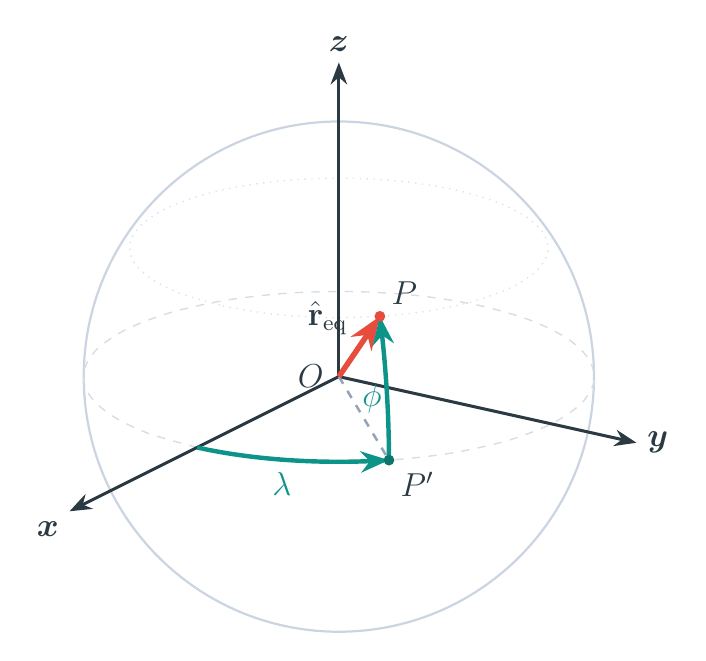
\begin{tikzpicture}[
    			scale=1.5, 
    			% Projection vectors giving a true circular sphere boundary
    			x={(-0.6cm,-0.3cm)}, 
    			y={(0.9cm,-0.2cm)}, 
    			z={(0cm,0.95cm)},
    			>=Stealth
    			]
    			
    			% Parameters
    			\def\alphaDeg{45}
    			\def\deltaDeg{35}
    			\def\R{2.0}
    			\pgfmathsetmacro{\Rproj}{\R*cos(\deltaDeg)}
    			
    			% Coordinates
    			\coordinate (O)  at (0,0,0);
    			\coordinate (X)  at (3.8,0,0);
    			\coordinate (Y)  at (0,2.8,0);
    			\coordinate (Z)  at (0,0,2.8);
    			
    			\coordinate (P)  at ({\Rproj*cos(\alphaDeg)}, {\Rproj*sin(\alphaDeg)}, {\R*sin(\deltaDeg)}); 
    			\coordinate (PP) at ({\R*cos(\alphaDeg)}, {\R*sin(\alphaDeg)}, 0);
    			
    			% Colors
    			\definecolor{axisColor}{HTML}{2B3A42}
    			\definecolor{vectorColor}{HTML}{E74C3C}
    			\definecolor{arcColor}{HTML}{0D9488}
    			\definecolor{guideColor}{HTML}{94A3B8}
    			\definecolor{sphereGrid}{HTML}{CBD5E1}
    			
    			% Background: Sphere Boundary Circle & Equatorial Circle
    			\begin{scope}%[on background layer]
    				% Outer sphere circle outline
    				\draw[sphereGrid, line width=0.8pt] (O) circle (1.08*\R cm);
    				
    				% Equatorial circle on sphere
    				\draw[sphereGrid!80, dashed, line width=0.5pt] plot[domain=0:360, variable=\t, smooth] 
    				({\R*cos(\t)}, {\R*sin(\t)}, 0);
    				
    				% Latitude parallel at angle \delta
    				\draw[sphereGrid!70, dotted, line width=0.5pt] plot[domain=0:360, variable=\t, smooth] 
    				({\Rproj*cos(\t)}, {\Rproj*sin(\t)}, {\R*sin(\deltaDeg)});
    			\end{scope}
    			
    			% Axes
    			\draw[->, axisColor, line width=1.1pt] (O) -- (X) node[below left, font=\large\bfseries] {$\boldsymbol{x}$};
    			\draw[->, axisColor, line width=1.1pt] (O) -- (Y) node[right, font=\large\bfseries] {$\boldsymbol{y}$};
    			\draw[->, axisColor, line width=1.1pt] (O) -- (Z) node[above, font=\large\bfseries] {$\boldsymbol z$};
    			\node[axisColor, left=2pt, font=\large\bfseries] at (O) {$O$};
    			
    			% Reference line to P'
    			\draw[dashed, guideColor, line width=0.9pt] (O) -- (PP);
    			
    			% Radius vector r_eq
    			\draw[->, vectorColor, line width=2.0pt] (O) -- (P) 
    			node[midway, above left, font=\large, color=axisColor] {$\hat{\mathbf{r}}_{\rm eq}$};
    			
    			% Spherical Arc  (Equator)
    			\draw[->, arcColor, line width=1.6pt] plot[domain=0:\alphaDeg, variable=\t, smooth]
    			({\R*cos(\t)}, {\R*sin(\t)}, 0);
    			\node[arcColor, font=\large\bfseries] at ({1.15*\R*cos(\alphaDeg/2)}, {1.15*\R*sin(\alphaDeg/2)}, -0.1) {$\lambda$};
    			
    			% Spherical Arc \delta (Meridian)
    			\draw[->, arcColor, line width=1.6pt] plot[domain=0:\deltaDeg, variable=\t, smooth]
    			({\R*cos(\t)*cos(\alphaDeg)}, {\R*cos(\t)*sin(\alphaDeg)}, {\R*sin(\t)});
    			\node[arcColor, font=\large\bfseries] at ($(PP)!0.5!(P)+(0.25,0.05,0)$) {$\phi$};
    			
    			% Points P and P'
    			\fill[vectorColor] (P) circle (1.3pt) node[above right=1pt, font=\large\bfseries, color=axisColor] {$P$};
    			\fill[arcColor!80!black] (PP) circle (1.3pt) node[below right=1pt, font=\large\bfseries, color=axisColor] {$P'$};
    		\end{tikzpicture}
\end{document}
